% =========================================================================== %
% Preamble                                                                    %
% =========================================================================== %

\documentclass[12pt, dvipsnames]{beamer}
%\documentclass[12pt, dipsnames, notes=only]{beamer}

\usepackage[utf8]{inputenc}
\usepackage{beamerthemesimple}

\title{bpfbox: Simple Precise Process Confinement in eBPF}
\author{\textbf{William Findlay} \and Anil Somayaji \and David Barrera}
\institute{Carleton University\\\url{will@ccsl.carleton.ca}}

\usepackage{csquotes}
\usepackage{booktabs}

% Center floats by default
\makeatletter
\g@addto@macro\@floatboxreset{\centering}
\makeatother

\usepackage{listings}

\definecolor{listing-background}{HTML}{F7F7F7}
\definecolor{listing-rule}{HTML}{B3B2B3}
\definecolor{listing-numbers}{HTML}{B3B2B3}
\definecolor{listing-text-color}{HTML}{000000}
\definecolor{listing-keyword}{HTML}{435489}
\definecolor{listing-keyword-2}{HTML}{1284CA} % additional keywords
\definecolor{listing-keyword-3}{HTML}{9137CB} % additional keywords
\definecolor{listing-identifier}{HTML}{435489}
\definecolor{listing-string}{HTML}{00999A}
\definecolor{listing-comment}{HTML}{8E8E8E}

% Set default listings style
\lstdefinestyle{listingstyle}{
    %backgroundcolor  = \color{listing-background},
    %xleftmargin      = 2em,
    numberstyle      = \color{listing-numbers}\ttfamily\normalsize\lst@ifdisplaystyle\footnotesize\fi,
    basicstyle       = \ttfamily\normalsize\lst@ifdisplaystyle\footnotesize\fi,
    keywordstyle     = {\color{listing-keyword}\bfseries},
    keywordstyle     = {[2]\color{listing-keyword-2}\bfseries},
    keywordstyle     = {[3]\color{listing-keyword-3}\bfseries\itshape},
    sensitive        = true,
    commentstyle     = \color{listing-comment},
    stringstyle      = \color{listing-string},
    showstringspaces = false,
    literate = {~}{$\sim$}{1}
}
\lstset{style=listingstyle}

\usepackage{bpfbox}

% Table of Contents for sections
\AtBeginSection[]
{
    \begin{frame}[noframenumbering, plain]
    %    \frametitle{Outline of Talk}
    %    \tableofcontents[currentsection]
        \begin{center}
        {\fontsize{42.99}{48}\selectfont \color{destacado} \insertsection}
        \end{center}
    \end{frame}
}

\def\vfilll{\vskip 0pt plus 1filll minus 0pt}

% =========================================================================== %
% Document                                                                    %
% =========================================================================== %

\begin{document}

%\setwatermark[hoffset=6cm, voffset=0.3cm]{
\includegraphics[height=1.5cm]{figs/carleton.pdf}}

% Title page
\begin{frame}[noframenumbering, plain]
\titlepage
\end{frame}

\setwatermark[hoffset=6cm, voffset=0.3cm]{}

% - bpfbox logo

\begin{frame}[noframenumbering, plain]{Outline of Talk}
    \tableofcontents
\end{frame}

\section{What is eBPF?}

\begin{frame}[c]{eBPF in the Beginning}
eBPF $\equiv$ \textbf{E}xtended \textbf{B}erkley \textbf{P}acket \textbf{F}ilter...
\begin{itemize}
    \item But it has little to do with Berkley, packets, or filtering nowadays
\end{itemize}
\vfill
So then \textbf{what is eBPF?}
\begin{itemize}
    \item A major re-write of the Linux BPF engine
    \begin{itemize}
        \item Alexei Starovoitov and Daniel Borkman
    \end{itemize}
    \item Merged into the Linux kernel in 2014
    \item The point was fine-grained, cross-layer \textbf{system introspection}
\end{itemize}
\end{frame}

\begin{frame}[t]{eBPF in 2020}
    \begin{itemize}
        \item
    \end{itemize}
\end{frame}

\section{Motivation}

% - Unix DAC, seccomp-bpf, namespaces, cgroups, Linux MAC (SELinux, AppArmor,
%   TOMOYO, etc.)
% - Where does this complexity arise from? No unified solution
% (Maybe the following can go into a separate slide...)
% - Higher level frameworks as Frankenstein's monster
% - Higher level frameworks being too coarse-grained (snap vs bpfbox)

\begin{frame}[t]{The Status Quo}
\begin{itemize}
    \item Existing process confinement mechanisms are \textbf{complex}
\end{itemize}
\begin{center}
    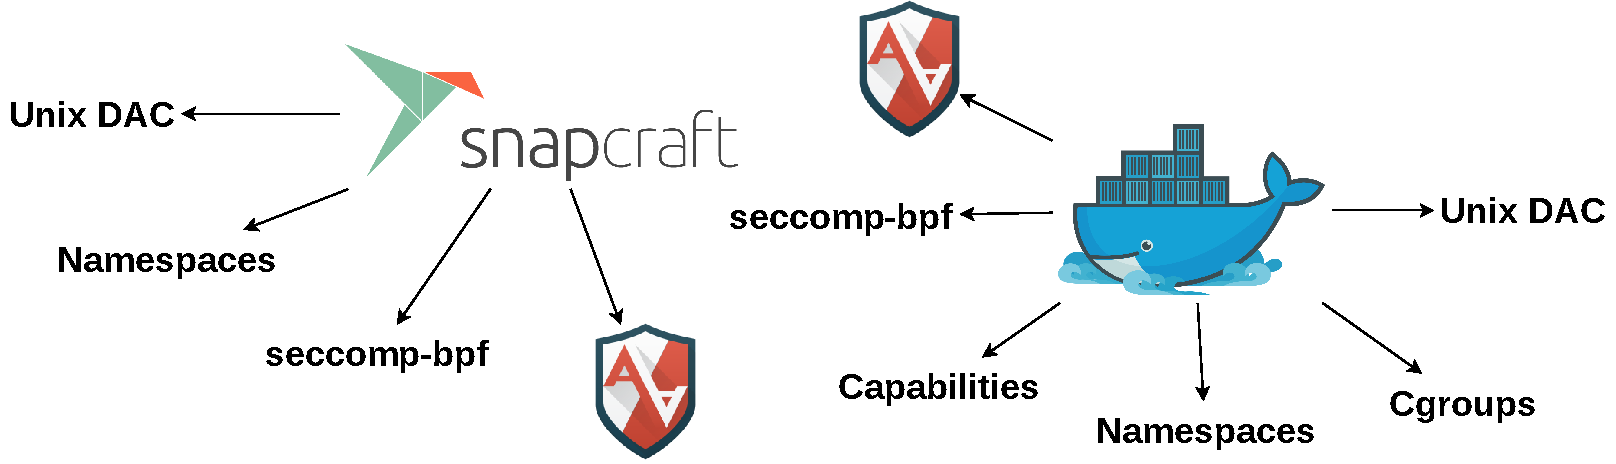
\includegraphics[width=0.8\textwidth]{figs/process-confinement-landscape.pdf}
\end{center}
\begin{itemize}
    \item Existing process confinement mechanisms are \textbf{difficult to use}
\end{itemize}
\begin{center}
    
\includegraphics[height=4em]{figs/selinux.png}
    \hspace{3em}
    
\includegraphics[height=4em]{figs/apparmor.png}
    \hspace{3em}
    
\includegraphics[height=4em]{figs/tomoyo.png}
\end{center}
%\begin{center}
%    \footnotesize (in order of decreasing difficulty)
%\end{center}
\begin{itemize}
    \item Can we do any better?
\end{itemize}
\end{frame}

% - Discuss all the access control mechanisms on Linux
% - Unix DAC, seccomp-bpf, namespaces, cgroups, Linux MAC (SELinux, AppArmor,
%   TOMOYO, etc.)
% - Where does this complexity arise from? No unified solution
% (Maybe the following can go into a separate slide...)
% - Higher level frameworks as Frankenstein's monster
% - Higher level frameworks being too coarse-grained (snap vs bpfbox)

\begin{frame}[t]{Stakeholders as Policy Authors}
\begin{itemize}
    \item \textbf{Security experts} define the policy
\end{itemize}
\begin{center}
    
\includegraphics[height=4em]{figs/selinux.png}
    \hspace{3em}
    
\includegraphics[height=4em]{figs/apparmor.png}
    \hspace{3em}
    
\includegraphics[height=4em]{figs/tomoyo.png}
\end{center}

\begin{itemize}
    \item \textbf{Application authors} and \textbf{packagers} define the policy
\end{itemize}
\begin{center}
    
\includegraphics[height=4em]{figs/snapcraft.png}
    \hspace{3em}
    
\includegraphics[height=4em]{figs/docker.png}
\end{center}

\begin{itemize}
    \item \textbf{End users} define the policy
\end{itemize}
\begin{center}
    \Huge ???
\end{center}
\end{frame}

% - Discuss stakeholders as policy authors:
% - security experts write policy and ship it with distributions
%   - SELinux, AppArmor, seccomp-bpf, etc.
% - application authors write policy and ship it with applications
%   - snap, etc.
% - end users write their own policy
%   - ???

\begin{frame}[t]{eBPF Changes the Game}
TODO
\end{frame}

\section{Architecture}

\begin{frame}[t]{bpfbox Architecture}
\begin{itemize}
    \item TODO: Python3 bcc
    \item TODO: KRSI
    \item TODO: Lines of userspace code
    \item TODO: Lines of kernelspace code
    \item TODO: Compare w/ SELinux, AppArmor
\end{itemize}
\end{frame}

\begin{frame}[t]{bpfbox Architecture}
\vfill
\begin{center}
    \color{black}
    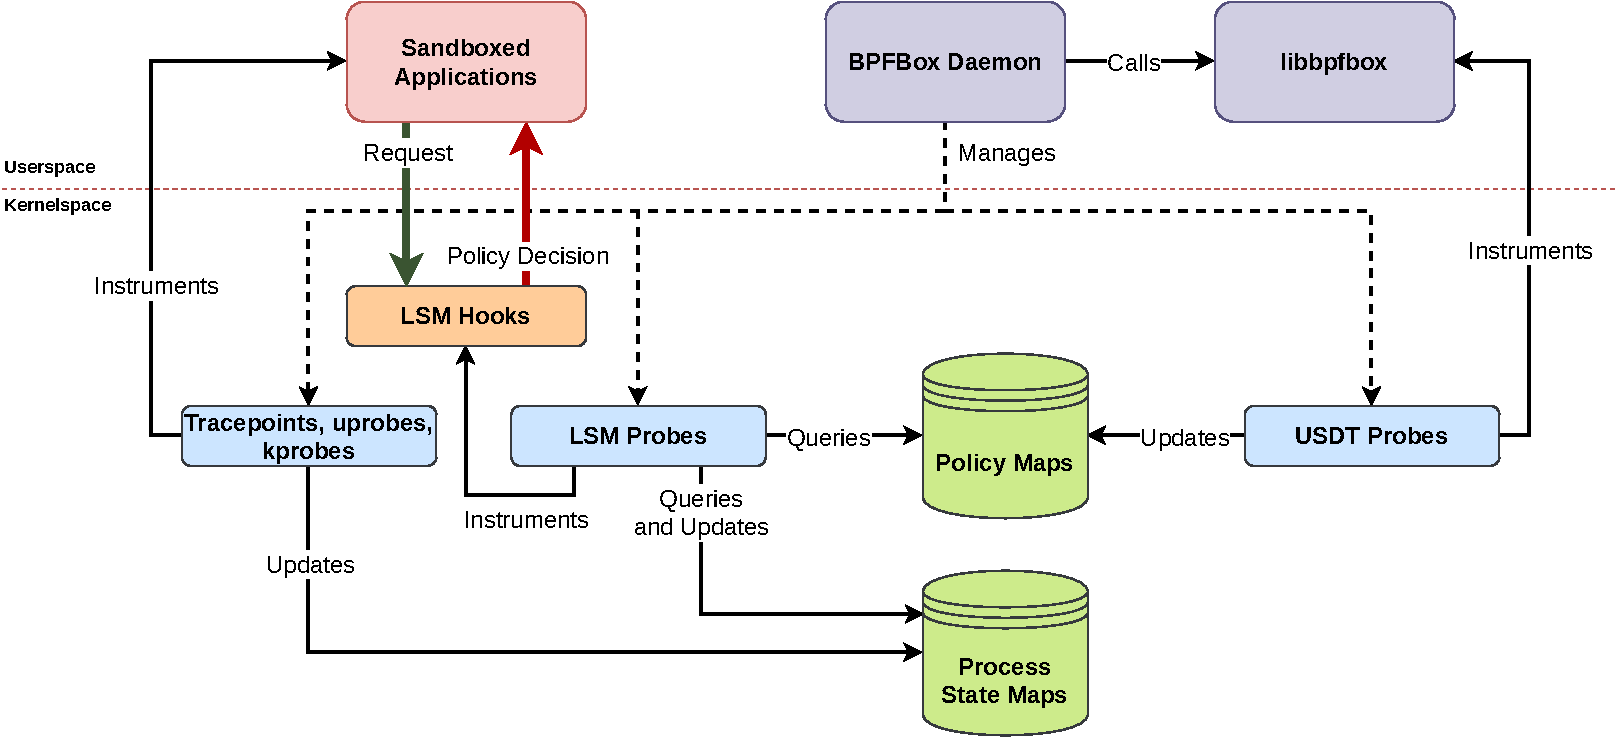
\includegraphics[width=0.9\textwidth]{figs/bpfbox-overview.pdf}
\end{center}
\vfill
\end{frame}

\section{Policy}

\begin{frame}[t, fragile]{Policy at the Function Call Level}
\begin{lstlisting}[language=bpfbox]
#![profile /sbin/mylogin]

#[func check_password]
#[func add_user]
#[allow] {
    read("/etc/passwd")
    read("/etc/shadow")
}

#[func add_user]
#[allow] {
    append("/etc/passwd")
    append("/etc/shadow")
}
\end{lstlisting}
\end{frame}

\section{Performance}

\begin{frame}[t]{Performance}
TODO
\end{frame}

\section{Conclusion}

\begin{frame}[t]{Acknowledgements}
TODO
\end{frame}

\begin{frame}[t]{Contributions}
\begin{itemize}
    \item First full policy enforcement engine written in eBPF
    \item Integration of \textbf{userspace} and \textbf{kernelspace} state with \textbf{LSM layer enforcement}
\end{itemize}
\end{frame}

\end{document}

% vim:syn=tex
